\documentclass[border=6pt]{standalone}
\usepackage{amsmath}
\usepackage{amssymb}
\usepackage{tikz}
\usepackage{xcolor}
\usetikzlibrary{arrows.meta,calc,positioning,shapes.geometric}
\begin{document}
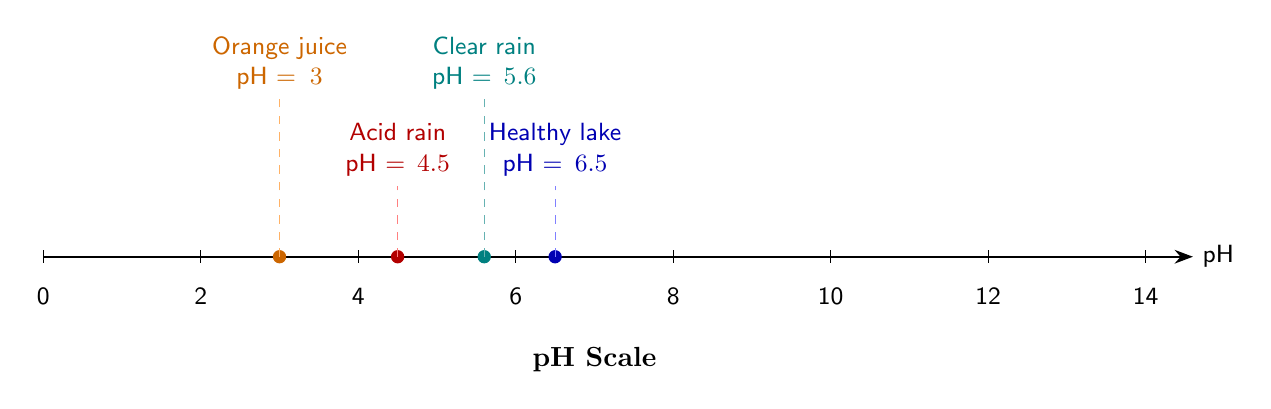
\begin{tikzpicture}[font=\sffamily\small]
  % pH axis
  \draw[thick, -Stealth] (0,0) -- (14.6,0);
  \node[right] at (14.6,0) {pH};
  \foreach \x in {0,2,4,6,8,10,12,14} {
    \draw (\x,0.08) -- (\x,-0.08);
    \node[below] at (\x,-0.28) {\x};
  }
  \node[font=\bfseries] at (7,-1.3) {pH Scale};

  % Orange juice, pH = 3 -- high label
  \filldraw[orange!80!black] (3,0) circle (2.2pt);
  \draw[orange!60, dashed] (3,0) -- (3,2.0);
  \node[above, text width=2.3cm, align=center, orange!80!black] at (3,2.0)
    {Orange juice\\ pH $=3$};

  % Acid rain, pH = 4.5 -- low label
  \filldraw[red!70!black] (4.5,0) circle (2.2pt);
  \draw[red!50, dashed] (4.5,0) -- (4.5,0.9);
  \node[above, text width=2.2cm, align=center, red!70!black] at (4.5,0.9)
    {Acid rain\\ pH $=4.5$};

  % Clear rain, pH = 5.6 -- high label
  \filldraw[teal] (5.6,0) circle (2.2pt);
  \draw[teal!60, dashed] (5.6,0) -- (5.6,2.0);
  \node[above, text width=2.2cm, align=center, teal] at (5.6,2.0)
    {Clear rain\\ pH $=5.6$};

  % Healthy lake, pH = 6.5 -- low label
  \filldraw[blue!70!black] (6.5,0) circle (2.2pt);
  \draw[blue!50, dashed] (6.5,0) -- (6.5,0.9);
  \node[above, text width=2.3cm, align=center, blue!70!black] at (6.5,0.9)
    {Healthy lake\\ pH $=6.5$};
\end{tikzpicture}
\end{document}
